\documentclass{article}
\usepackage[utf8]{inputenc}
\usepackage[english]{babel}
\usepackage[]{amsthm} %lets us use \begin{proof}
\usepackage[]{amssymb} %gives us the character \varnothing
\usepackage{amsmath}
\usepackage{algpseudocode}
\usepackage{graphicx}
\usepackage{hyperref}
\usepackage{hypcap}
\usepackage{float}


\title{RNA-seq Expectation Maximization}
\date{}
\author{Arush Ramteke}
\begin{document}
\maketitle

\section*{What I Did}

I implemented the IsoEM version of expectation maximization for quantifying RNA-Seq data \cite{nicolae}.

\subsection*{IsoEM}

IsoEM is an equivalence-class based implementation of EM that works with fully aligned and not pseudoaligned reads.
It assigns weights to each transcript-read pairing as follows, and performs the expectation step of the algorithm for each read with only transcripts with non-zero weights (effectively a weighted equivalence class). The weights can be thought of as the probability of a read given a transcript.

$$ w_{r,j} = \sum_{a}Q_aF_aO_a$$

Here, we compute the weight of transcript $j$ for read $r$ by summing over all possible alignments the terms:
\begin{itemize}
    \item{$Q_a$: this is effectively the quality of the alignment, and would traditionally be computed as the base quality probabilities (present in the BAM file) weighted by if the read matched the transcript at that position. \textbf{Here, we assume $Q_a = 1$ for all aligned reads.}}
    \item{$F_a$: for single end reads, this is the probablity of the fragment length being lower than some upperbound $u$. \textbf{Here, we assume $F_a = 1$ for all aligned reads.}}
    \item {$O_a$: this reflects if the orientation of the read matches the orientation of the original transcript. Since we don't care about direction in our case, \textbf{we assume $O_a$ = 1 for all aligned reads.}}
\end{itemize}

Hence, to compute weights for each transcript-read pairing, we simply count the number of alignments a particular read has with a transcript. For implementation purposes, we only need to store non-zero ones to save memory.

\break

Let $\theta$ be the vector of the relative abundances we are interested in, $c$ be the vector of the expected counts for each transcript, and $l$ be the vector of each transcript length. Let $mu$ be the upperbound on fragment length, which we set as 200. As probabilities, for transcript j and read r:
$$P(j) = \theta(j)$$
$$P(r|j) = w_{r,j}$$
$$P(r, j) = w_{r, j}\theta(j)$$
$$P(r) = \sum_{j}{P(r,j)} = \sum_{j}{w_{r,j}\theta(j)}$$
$$c(j) = E[j|r] = \sum_{r}{P(j|r)} = \sum_{r}{P(r,j)/P(j)}$$

The algorithm is thus as follows.\\

\begin{algorithmic}
    \State $\forall j, \theta(j) \gets 1/len(\theta)$
    \While{not converged} 
        \State \textbf{E-Step:} Determine expected counts $c$
        \State $\forall j, c \gets 0$
        \For{each read r}
            \State $P(r) \gets \sum_{j}{w_{r,j}f(j)}$
            \For{each transcript j}
                \State $P(r,j) \gets w_{r,j}f(j)$
                \State $c(j) \gets c(j) + P(r, j)/P(r)$
            \EndFor
        \EndFor
        \State \textbf{M-Step:} Re-assign relative abundances (normalized by transcript length)
        \State $total \gets \sum_{j}{c(j)/(l(j)-\mu + 1)}$
        \For{each transcript j}
            \State $\theta \gets (c(j)/(l(j)-\mu + 1))/total$
        \EndFor

    \EndWhile
\end{algorithmic}
\vspace{1em}
There are instances of transcripts with length shorter than 200. If this is the case, their relative abundance is set to 0.

\break
\subsection*{Implementation Details}

The main challenge in implementation was determining how computing weights. For this, I used a hash table of hash tables. The outer hash table is keyed by the read, and the inner hash table is keyed by the transcript ID. The values of the inner table are the weight itself, which is incremented if the key already exists, else is added as 1. This structure is not the most time efficient but considering the number of alignments (1282526) and the number of transcripts (7138), storing it in matrix form is unfeasible.
\\
The convergence criteria I used was median relative difference in the relative abundances between epochs. The threshold I set was 0.001.

\subsection*{Results}

The algorithm converged very fast, requiring 50 iterations and a total runtime of 4.5 minutes.

\begin{figure}[H]
    \centering
      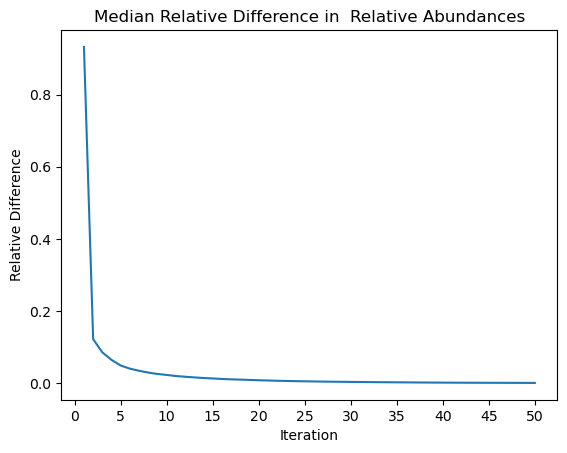
\includegraphics[width=0.8\linewidth]{./images/convergence.png}
  \caption{Convergence}\label{figure1}%
\end{figure}

The first 20 entries of the final results table are also shown in \autoref{table1}. This can be found in table.csv in the results directory.

\begin{figure}[H]
    \centering
      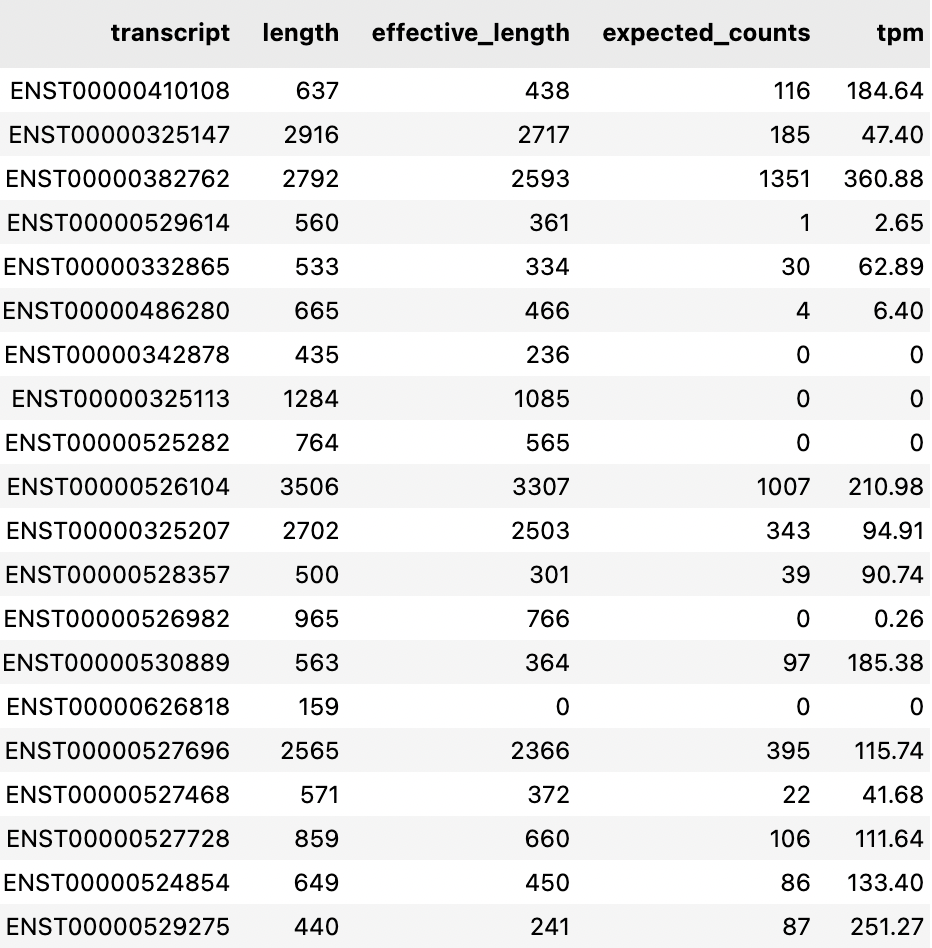
\includegraphics[width=0.8\linewidth]{./images/table.png}
  \caption{IsoEM Output}\label{table1}%
\end{figure}

\subsection*{Comparison with Kallisto}

I converted the unique reads in the BAM file to FASTQ format and ran Kallisto \cite{kallisto} on this data. Instead of taking a hard upper-bound on the fragment length, Kallisto requires a mean and standard deviation of fragment length which I passed as 200 and 3.16 (variance = 10).

Performing a simple eye test on the relative abundances and expected counts generally follow similar trends, but differ in absolute values. The median relative absolute error between Kallisto and IsoEM relative to kallisto is 0.325. While this is not very low, it is somewhat reasonable.

However, the mean relative absolute error is enormous, and is equal to 21083.15. Below, \autoref{figure2a} and \autoref{figure2b} are boxplots of the log relative absolute errors between Kallisto and IsoEM relative abundances with and without outliers included. It is clear that outliers have substantial effect, but I am not sure if that is due to an error in my implementation of IsoEM or minor differences in how certain edge cases are handled.

\begin{figure}[H]
    \centering
      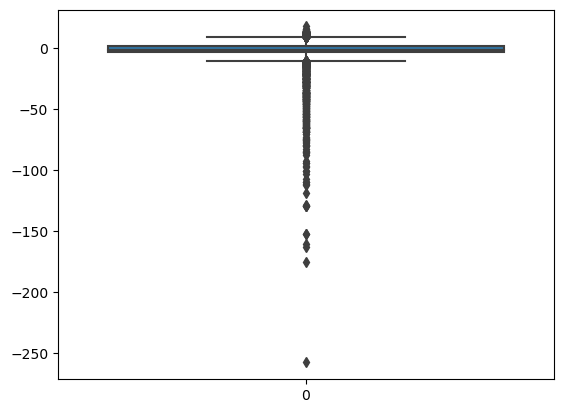
\includegraphics[width=0.8\linewidth]{./images/outliers.png}
  \caption{Log Relative Error vs Kallisto with Outliers}\label{figure2a}%
\end{figure}

\begin{figure}[H]
    \centering
      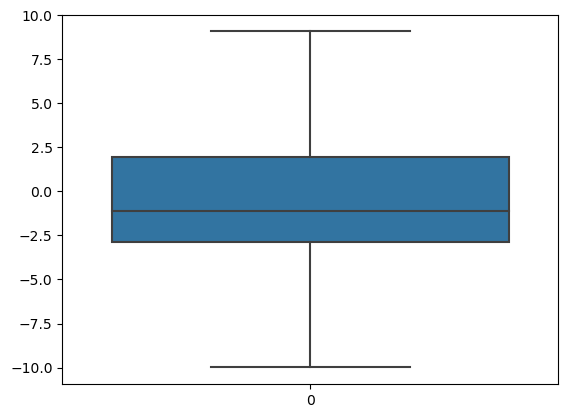
\includegraphics[width=0.8\linewidth]{./images/normal.png}
  \caption{Log Relative Error vs Kallisto without Outliers}\label{figure2b}%
\end{figure}




\clearpage
\begin{thebibliography}{9}
    \bibitem{nicolae}
    Nicolae, M., Mangul, S., Măndoiu, I.I. et al. Estimation of alternative splicing isoform frequencies from RNA-Seq data. Algorithms Mol Biol 6, 9 (2011). https://doi.org/10.1186/1748-7188-6-9

    \bibitem{kallisto}
    Bray, N., Pimentel, H., Melsted, P. et al. Near-optimal probabilistic RNA-seq quantification. Nat Biotechnol 34, 525–527 (2016). https://doi.org/10.1038/nbt.3519
\end{thebibliography}

\end{document}